\chapter{Additional Material} \label{app:additional}

\section{Parameters for the training in Nerfstudio} \label{sec:nerfstudio-train-parameters}

\subsection{Nerfacto}
\begin{table}[h]
    \begin{tabular}{|l|l|}
    \hline
    Description                                             & Default Value \\
    \hline
    How far along the ray to start sampling.                & 0.05 \\
    How far along the ray to stop sampling.                 & 1000.0 \\
    %Whether to randomize the background color.              & \"last\_sample\" \\
    %Number of samples per ray for the proposal network.     & \(256, 96\) \\
    Number of samples per ray for the nerf network.         & 48 \\
    Sample every n steps after the warmup                   & 5 \\
    Scales n from 1 to proposal\_update\_every over this many steps & 5000 \\
    Number of proposal network iterations.                  & 2 \\
    Use the same proposal network. Otherwise use different ones. & False \\
    Proposal loss multiplier.                               & 1.0 \\
    Distortion loss multiplier.                             & 0.002 \\
    Orientation loss multipier on computed noramls.         & 0.0001 \\
    Predicted normal loss multiplier.                       & 0.001 \\
    Whether to use proposal weight annealing.               & True \\
    Whether to use average appearance embedding or zeros for inference. & True \\
    Slope of the annealing function for the proposal weights & 10.0 \\
    Max num iterations for the annealing function.          & 1000 \\
    Whether use single jitter or not for the proposal networks. & True \\
    Whether to predict normals or not.                      & False \\
    \hline
    \hline
    Description of corresponding proposal density fields    & Default Value \\
    \hline
    Dimension of hidden layer           & 16 \\
    Hashmap size                        & $2^{17}$ \\
    Number of levels of the hashmap     & 5 \\
    Maximum resolution of the hashmap (density field 1)         & 64 \\
    Maximum resolution of the hashmap (density field 2)         & 256 \\
    \hline
    \end{tabular}
    \caption{An overview of the parameters in the default Nerfacto model}
    \label{tab:nerfacto-parameter-overview}
\end{table}

\subsection{Instant-ngp}
\begin{table}[h]
    %\centering
    \begin{tabular}{|l|l|}
    \hline
    \textbf{Description} & \textbf{Value} \\ 
    \hline
    Whether to create a scene collider to filter rays. & False \\
    Number of samples in field evaluation. & 24 \\
    Resolution of the grid used for the field. & 128 \\
    Contraction type. & Unbounded Sphere \\
    Cone angle & 0.004 \\
    Minimum step size for rendering. & 0.01 \\
    How far along ray to start sampling. & 0.05 \\
    How far along ray to stop sampling. & 1e3 \\
    Whether to use an appearance embedding. & False \\
    Whether to randomize the background color. & True \\ \hline
    \end{tabular}
    \caption{An overview of the parameters in the default Instant-ngp model}
    \label{tab:instant-ngp-parameter-overview}
\end{table}

\subsection{NeRF}
\begin{table}[h]
    %\centering
    \begin{tabular}{|l|l|}
    \hline
    \textbf{Description} & \textbf{Value} \\ 
    \hline
    Number of samples in coarse field evaluation & 64 \\
    Number of samples in fine field evaluation & 128 \\
    Specifies whether or not to include ray warping based on time. & False \\
    \hline
    \end{tabular}
    \caption{An overview of the parameters in the default NeRF model}
    \label{tab:nerf-parameter-overview}
\end{table}

\subsection{mip-NeRF}
\begin{table}[h]
    %\centering
    \begin{tabular}{|l|l|}
    \hline
    \textbf{Description} & \textbf{Value} \\ 
    \hline
    Whether to create a scene collider to filter rays.  & True \\
    Near plane collider-plane.                          & 2.0 \\
    Far plane collider-plane.                           & 6.0 \\
    The loss coeficcient for the coarse MLP.            & 1.0 \\
    The loss coeficcient for the fine MLP.              & 1.0 \\
    Number of rays per chunk during eval                & 4096 \\
    \hline
    \end{tabular}
    \caption{An overview of the parameters in the default mip-NeRF model}
    \label{tab:mip-nerf-parameter-overview}
\end{table}


\begin{comment}
    
Additional material that does not fit in the main thesis but may still be relevant to share, e.g., raw data from experiments and surveys, code listings, additional plots, pre-project reports, project agreements, contracts, logs etc., can be put in appendices. Simply issue the command \texttt{\textbackslash appendix} in the main \texttt{.tex} file, and make one chapter per appendix.

If the appendix is in the form of a ready-made PDF file, it should be supported by a small descriptive text, and included using the \texttt{pdfpages} package. To illustrate how it works, a standard project agreement (for the IE faculty at NTNU in Gjøvik) is attached here. You would probably want the included PDF file to begin on an odd (right hand) page, which is achieved by using the \texttt{\textbackslash cleardoublepage} command immediately before the \texttt{\textbackslash includepdf[]\{\}} command. Use the option \texttt{[pages=-]} to include all pages of the PDF document, or, e.g., \texttt{[pages=2-4]} to include only the given page range.

\cleardoublepage
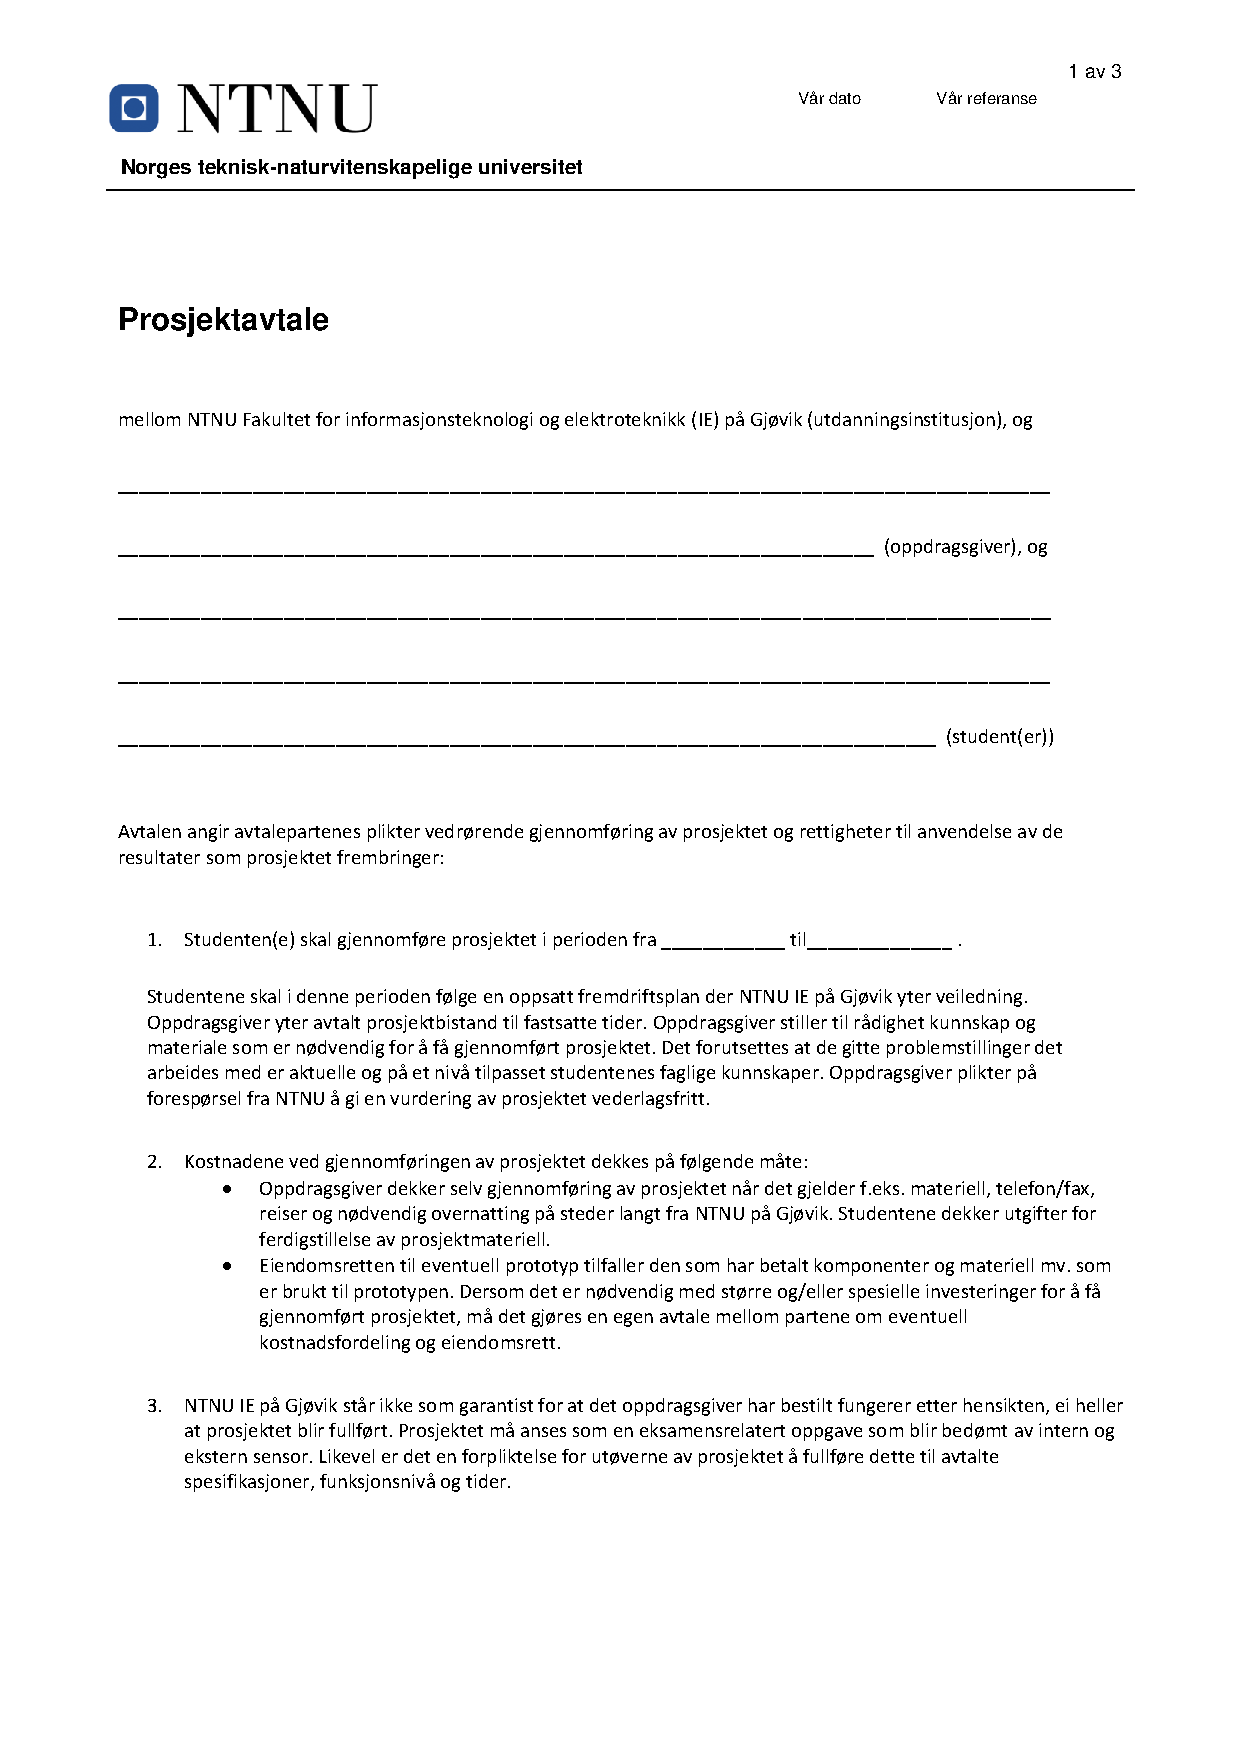
\includepdf[pages=-]{appendices/NTNUProsjektavtale.pdf}
\end{comment}

\begin{figure}[h]
    \centering
    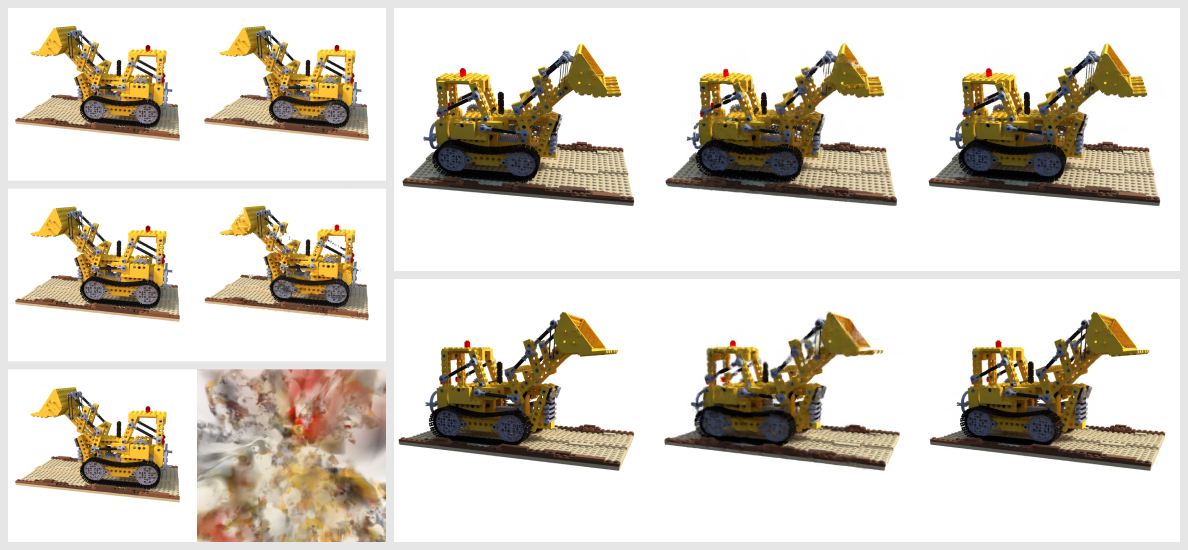
\includegraphics[width=1.0\textwidth]{figures/lego-result.png}
    \caption{Evaluation image is the left-most image per each experiment.
    Left column, top to bottom: 1) instant-ngp, 2) Nerfacto (adjusted), 3) Nerfacto (unadjusted). Right column, top to bottom: 4) mip-NeRF with both the coarse and fine RGB output, 5) NeRF with both the coarse and fine RGB output}
    \label{fig:lego-result}
\end{figure}
\begin{figure}[h]
    \centering
    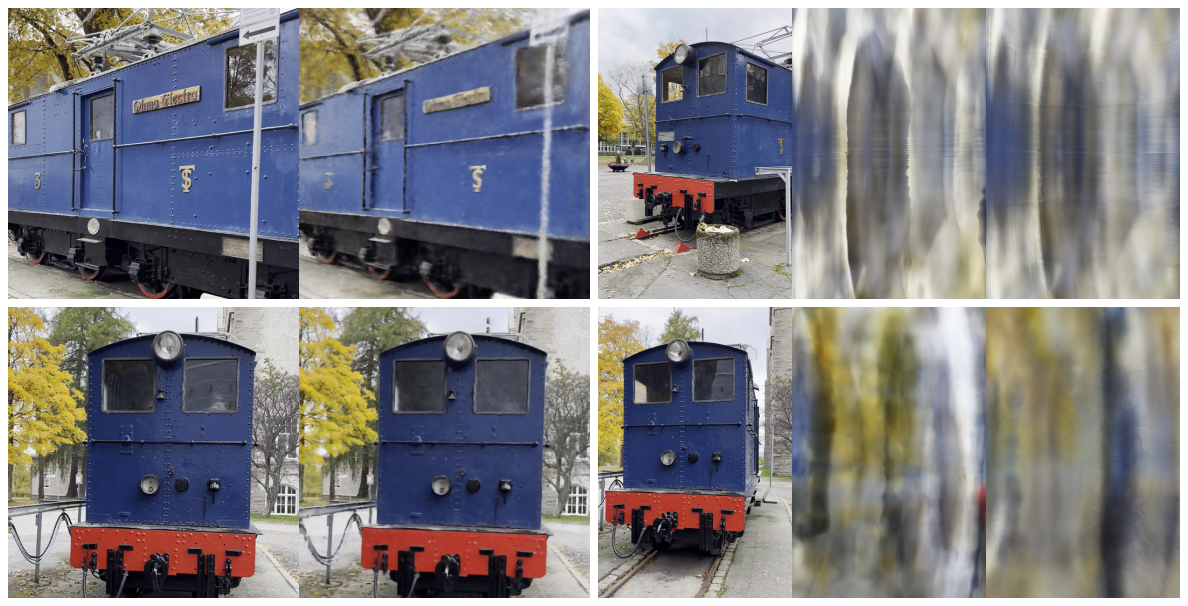
\includegraphics[width=1.0\textwidth]{figures/ohma-electra-result.png}
    \caption{Evaluation image is the left-most image per each experiment.
    Left column, top to bottom: 1) Instant-ngp, 2) Nerfacto. Right column, top to bottom: 3) Mip-NeRF with both the coarse and fine RGB output, 4) NeRF with both the coarse and fine RGB output}
    \label{fig:ohma-electra-result}
\end{figure}
\begin{figure}[h]
    \centering
    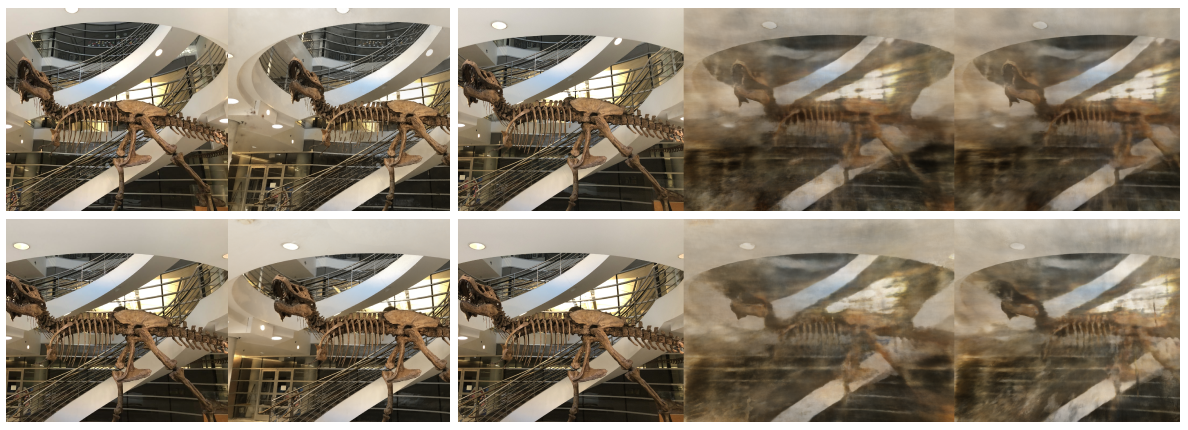
\includegraphics[width=1.0\textwidth]{figures/trex-result.png}
    \caption{Evaluation image is the left-most image per each experiment.
    Left column, top to bottom: 1) instant-ngp, 2) Nerfacto. Right column, top to bottom: 3) mip-NeRF with both the coarse and fine RGB output, 4) NeRF with both the coarse and fine RGB output}
    \label{fig:trex-result}
\end{figure}